\section{Machine Learning Method}

For the machine learning method, the library Weka, developed at the University of Waikato in New Zealand, was chosen. As described by Witten et al., "the Weka workbench is a collection of machine learning algorithms and data preprocessing tools" \cite[p.~7]{Weka}. It includes tools for the entire process of data mining, such as preparation of data and evaluation. Weka is implemented in Java, the version used in this thesis was 3.9.6. Although it also offers a graphical interface, only the Java library was used in this thesis \cite{Weka}. Weka was chosen because of its large collection of both algorithms and tools for data mining, as well as ease of use through an extensive documentation.

Weka uses the Attribute-Relation File Format for its data, which contains a header describing the attributes, as well as the data itself, with one row containing one instance \cite{Weka}. For this thesis, the class attribute was chosen to be nominal, either negative (-1.0) or positive (1.0), in order to implement sentiment polarity classification. The tweet text was added as a string attribute.

\subsection{Training Data}
The training data for machine learning classifiers was created by Go et al. and consists of 1.6 million tweets \cite{GoBHaHua2009}. As mentioned previously in section \ref{sub:related_ml}, the tweets were parsed using the Twitter API by querying for positive or negative emoticons, such as ":)", and labeled accordingly. Furthermore, tweets containing both a negative and positive emoticon, as well as retweets were removed. The emoticons were also removed from the tweets, as the emoticons had a negative effect on classification \cite{GoBHaHua2009}.

This resulted in 800,000 positive and 800,000 negative tweets that were periodically requested from April to June 2009 on no specific topic, thus covering a large number of topics \cite{GoBHaHua2009}.

\subsection{Preprocessing}

\subsubsection{URL/Hashtag Removal}
The hashtag character and URLs were removed using regular expressions.

\subsubsection{Stop Word Filtering}
For stop word filtering, both a list and a dynamic approach were implemented. A short list of common words, such as "the", was manually collected. To further reduce the word size, a limit was set for how often a word has to appear to be included, as well as a soft limit of total words. In testing, a limit of 15,000 words was found to be optimal, with words appearing at least 20 times in the training data. This allowed for the greatest balance of performance and accuracy. The limit was set in Weka's "StringToWordVector", which is explained in more detail in section \ref{sub:feature_selec}.

\subsubsection{Stemming}
For stemming, Weka's "LovinsStemmer" was used, which is based on the Lovins Stemmer \cite{Weka}. This stemmer uses a two-step method, which first removes the ending, thus obtaining the stem. After this, similar stems are combined to account for different spellings. An example of this is "absorption", whose stem is "absorpt", while "absorbing" will result in "absorb" \cite{Lovins1968DevelopmentOA}.

\subsection{Feature Selection}
\label{sub:feature_selec}


In order to transform the text of a tweet into features, and thus a suitable format for classifiers, Weka's "StringToWordVector" filter was used. This filter transforms the string feature, the tweet's text, by parsing each word out of it. This process is also known as tokenization \cite{DBLP:journals/csur/GiachanouC16}, which was implemented using Weka's "NGramTokenizer". This class splits a text into n-grams of a certain size. Standard delimiters, such as whitespace and "\textbackslash n", were used for splitting. The minimum and maximum size of n-grams were set according to whether a unigram, bigram, or the combination was used \cite{Weka}. Additionally, the filter converted all terms to lowercase and automatically added all recognized terms to a dictionary. In the filtered data, the terms were implemented as numeric attributes, with the value denoting the number of occurrences or their presence, based on the setting \cite{Weka}.

For example, the tweet "i love it" would result in three attributes, the attribute "i", the attribute "love", and the attribute "it", as can be seen in Figure \ref{fig:arff_train}. The values denote the attribute index and the number of occurrences in the tweet. For example, the attribute "i" has the index 1 and appears once in the document, resulting in the value "1 1". The dictionary, and thus the attributes, were all determined by the training data. The test data set was also filtered, but only using the known words from the training data, no new words were added to the dictionary \cite{Weka}.

\begin{figure}
    \centering
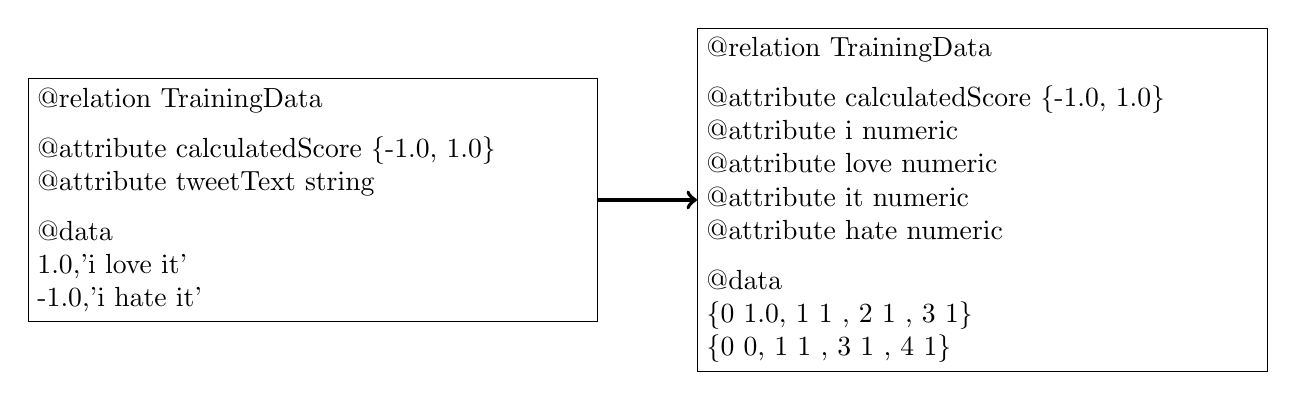
\begin{tikzpicture}
\vspace{5mm}
\node[draw, text width=7cm](A) at (0,0) { @relation TrainingData \\
                                        \medskip
                                        @attribute calculatedScore \{-1.0, 1.0\} \\
                                        @attribute tweetText string \\
                                        \medskip
                                        @data \\
                                        1.0,'i love it' \\
                                        -1.0,'i hate it' \\
                                        
                                        };
\node[draw, text width=7cm](B) at (8.5,0) { @relation TrainingData \\
                                        \medskip
                                        @attribute calculatedScore \{-1.0, 1.0\} \\
                                        @attribute i numeric \\
                                        @attribute love numeric \\
                                        @attribute it numeric \\
                                        @attribute hate numeric \\
                                        \medskip
                                        @data \\
                                        \{0 1.0, 1 1 , 2 1 , 3 1\} \\
                                        \{0 0,   1 1 , 3 1 , 4 1\}
                                        };
\draw[->, line width=0.5mm] (A) -- (B);

\end{tikzpicture}
\vspace{1mm}
    \caption{Example of training data in the ARFF format utilized by Weka before and after feature selection.}
    \label{fig:arff_train}
\end{figure}

\subsection{Training}
For training, Weka's "FilteredClassifier" was used, which combines an arbitrary filter with an arbitrary classifier. The classifier classes used were (1) "NaiveBayes" for Gaussian Naive Bayes, (2) "NaiveBayesMultinomial" for Multinomial Naive Bayes, (3) "Logistic" for Logistic Regression, (4) "LibSVM" for Support Vector Machine, and (5) "RandomForest" for Random Forest \cite{Weka}. For Support Vector Machine, the LibSVM library \cite{Chang2001} had to be added to the project, as Weka only provides a wrapper class. Once a classifier was built, its file was saved. Random Forest resulted in large files, with the largest being 471 megabytes. For evaluation, Weka's "Evaluation" class was used, which is able to calculate all necessary measures \cite{Weka}.